\documentclass[12pt]{article}

\usepackage{listings}
\usepackage{xcolor}
\usepackage{graphicx}
\usepackage[top=2cm,bottom=2cm,left=3cm, right=3cm]{geometry}
\usepackage{float}

\lstset{
basicstyle=\scriptsize\tt,
  backgroundcolor=\color{gray!10},
  commentstyle=\color{green!60!black},
  keywordstyle=\color{blue},
  stringstyle=\color{orange},
  numbers=left,
  numbersep=5pt,
  numberstyle=\tiny\color{gray},
}



\title{Report on Partitioning Clustering and  Energy Forecasting}
\newcommand{\name}{Hasanur Rahman Mohammad}
\newcommand{\studentID}{w1780941}
\newcommand{\moduleCode}{5DATA002W}
\newcommand{\tutor}{Mahmoud Aldraimli}
\newcommand{\seminarGroup}{5CS01}
\setlength{\parindent}{0pt}

\begin{document}
\begin{titlepage}

    \center
    {\LARGE\bfseries Report on Partitioning Clustering and Energy Forecasting}
    \\ [2cm]
    \begin{flushleft}
        \textbf{Name: }\name \\
        \textbf{Student ID: }\studentID \\[0.5cm]
        \textbf{Module Code: }\moduleCode \\
        \textbf{Tutor: }\tutor \\
        \textbf{Seminar Group: }\seminarGroup\\
    \end{flushleft}

\end{titlepage}

\tableofcontents
\newpage

\section{Partitioning Clustering}
\subsection{Pre-Processing the data}
For this task we were given a vehicle.xmls file containing \textbf{846} samples, with \textbf{19} different attributes
including the \textbf{'Class'}. However, as the goal is to perform k-means clustering on the data, an unsupervised learning algorithm,
it is required to remove the \textbf{'Class'} column as the model will classify the data on its own. I also removed the 'Sample' column as it will
affect the next pre-processing tasks, scaling and outlier removal.\\

When it comes to the order, I chose to remove the outliers first as they seemed to negatively affect the clustering results if I scaled the data before removing them.
To find the outliers I found the \textbf{z-score} for each of the samples and then removed any samples with a \textbf{z-score} than \textbf{3} and less than \textbf{-3}.

\subsection{Finding the best k using: Nblust, Elbow method, Gap statistics and sillhoutte methods}

\subsubsection{Nblust}
As shown below, Nbclust says the best number of clusters is 3. Considering the original number of classes is 4 I believe that this is a good result.
\begin{lstlisting}
* Among all indices:                                                
* 6 proposed 2 as the best number of clusters 
* 12 proposed 3 as the best number of clusters 
* 1 proposed 6 as the best number of clusters 
* 1 proposed 8 as the best number of clusters 
* 1 proposed 11 as the best number of clusters 
* 1 proposed 12 as the best number of clusters 
* 2 proposed 15 as the best number of clusters 

                   ***** Conclusion *****                            
 
* According to the majority rule, the best number of clusters is  3 
\end{lstlisting}

\subsubsection{Elbow Method}
\begin{figure}[H]
  \centering
  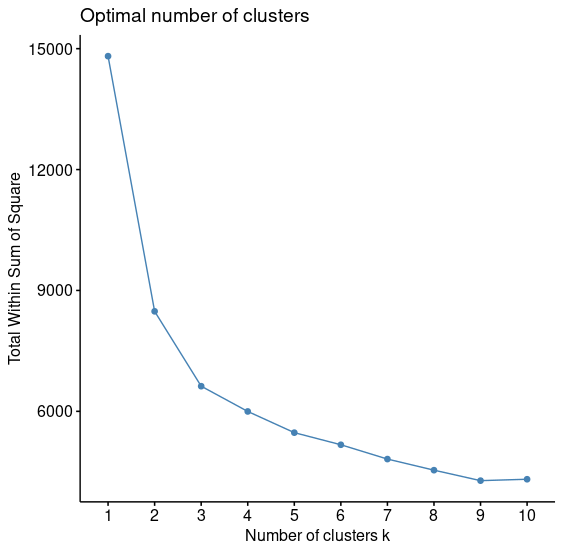
\includegraphics[width=0.5\textwidth]{~/Documents/rcw/images/Rplot.png}
  \caption{Elbow method plot}
\end{figure}

The Elbow method uses the \textbf{WCSS(within-cluster sums of squares)} which measueres how close data points are in respect of their cluster centers.
Based on the plot above, the reccomended number of clusters is \textbf{3} as that is where the results begin to flatten out slowly
indicating that increasing the clusters anymore will not result in any increase in performance.

\subsubsection{Gap Statistics}
\begin{figure}[H]
  \centering
  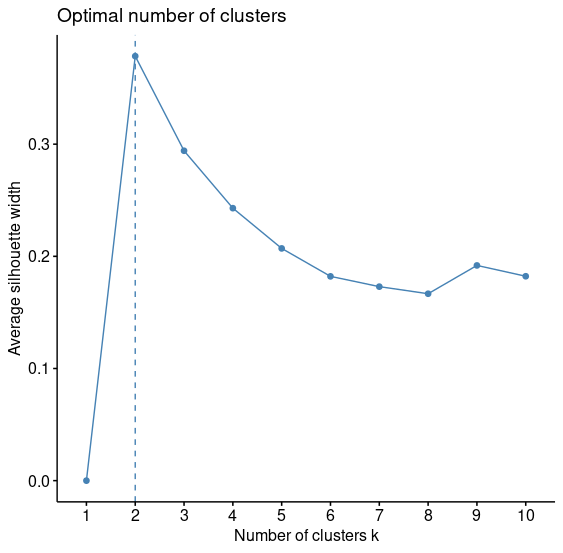
\includegraphics[width=0.5\textwidth]{~/Documents/rcw/images/Rplot01.png}
  \caption{Gap statistics plot}
\end{figure}

The Gap statistics also uses the \textbf{WCSS} to calculate the best number of clusters to use.  
However, the reccomended number of clusters in this case is \textbf{2}, knowing that the orignal data set has \textbf{4} possible classes,
we can conclude that this result is worse than what we got with the elbow method which was \textbf{3}.

\subsubsection{Sillhoutte  Method}
\begin{figure}[H]
  \centering
  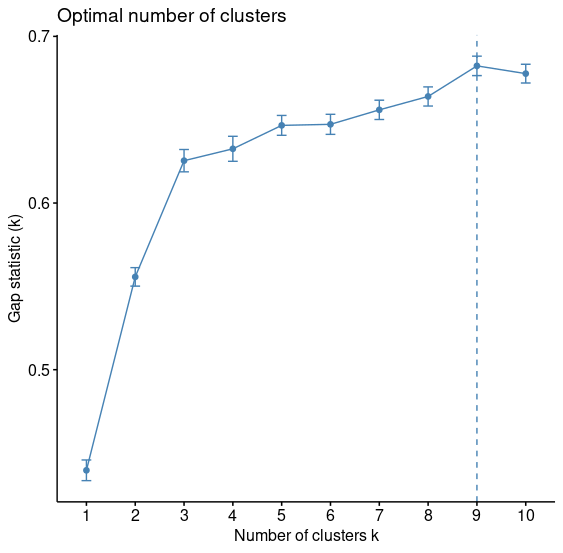
\includegraphics[width=0.5\textwidth]{~/Documents/rcw/images/Rplot02.png}
  \caption{Sillhoutte method plot}
\end{figure}

The sillhoutte plot shows how similar a data point is to its own cluster using the \textbf{sillhuotte score}, this is a value 
that ranges from -1 and 1, with values closer to -1 meaning the data point should be in another cluster and the closer the value is to 1 meaning the current cluster is a good fit for the data point
This is where things get interesting, based on the plot above \textbf{9} is the reccomended number of clusters. This is significantly higher
than any of the other results from the other evaluation methods,
I made to sure to run the model several times checking if there were errors with the code, but it gave \textbf{9} as the ouput everytime. This is by far the worst result as the orignal data set has \textbf{4} classes

However as shown later in the report, after running the evaluation tools for the data that had \textbf{PCA} done on it. The results for the sillhoutte plot were 
a lot more controlled and matched the other evaluation methods as well. This led me to believe that having a data set that is too multi-demensional led to an extreme result for the sillhoutte plot.

\newpage
\subsection{K-means Clustering investigation}
Using the results from the evaluation methods, I decided to go for \textbf{k=3}, as both \textbf{Nbclust} and the \textbf{Elbow Method} \
gave a result of the best \textbf{k} being \textbf{3}.
Below you can see the plot made from the clustering, without looking at the output data you can see a clear distinction between the clusters where there is 
no overlapping

\begin{figure}[H]
  \centering
  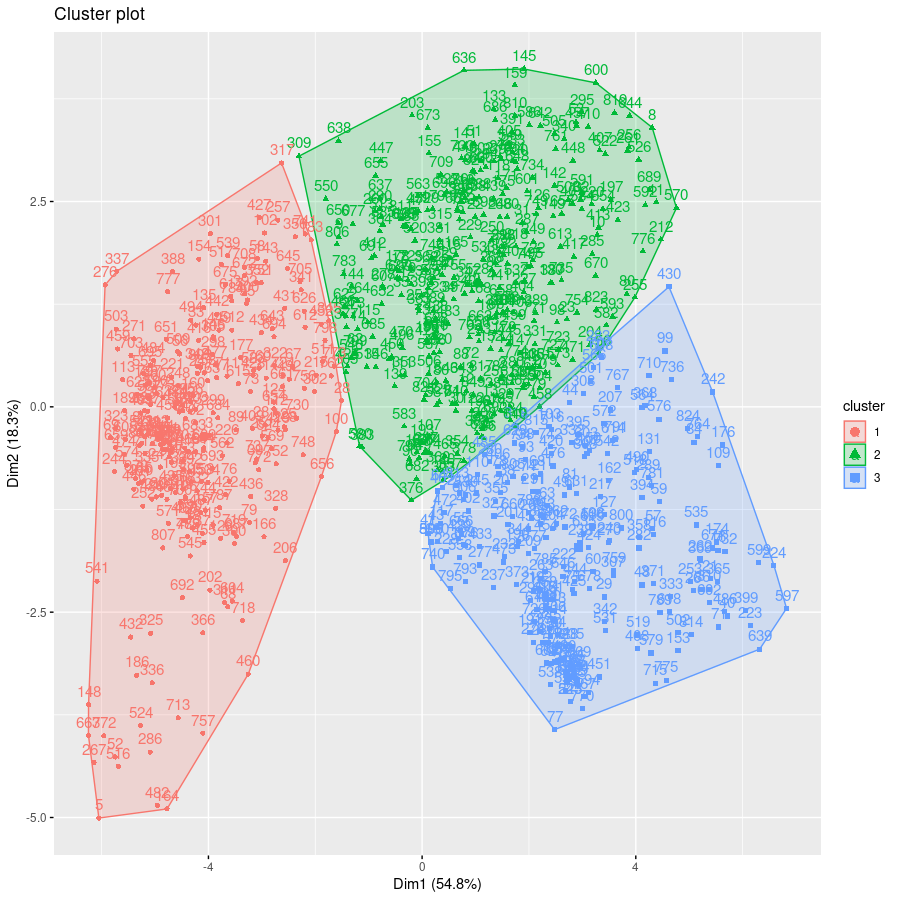
\includegraphics[width=0.8\textwidth]{~/Documents/rcw/images/Rplot05.png}
  \caption{Clustering plot}
\end{figure}

Below are the kmeans output for the clustering attempt with \textbf{k=3}. First of all you can see that the sizes of each cluster is evenly distributed
which means there isn't a cluster that has too many or too little data samples.





\lstinputlisting{tools.txt}


\end{document}


